\documentclass[12pt,parskip]{scrartcl}

\usepackage[utf8]{inputenc}
\usepackage[T1]{fontenc}
\usepackage[ngerman]{babel}

\usepackage{pdfpages}
\usepackage{tikz}
\usetikzlibrary{calc}


\title{Veranstaltung -- Blatt X}
\author{Name Y, Name Z}
\date{\today}



\begin{document}
\maketitle
\thispagestyle{empty}

\vspace{7cm}

% Set Number of excercises
\newcommand*{\numExcersises}{4}
\newcommand*{\scaleTable}{1}



\begin{center}
  \begin{tikzpicture}[scale=\scaleTable]
    \draw[very thick]  (0, 0) -- ($2*(\numExcersises,0) + (2,0)$);
    \foreach \x in {2,..., \numExcersises}{
      \draw  ($2*(\x,0) + (-2, 1.5)$) -- ($2*(\x,0) + (-2, -1.5)$);
    }
    \draw[very thick]  ($2*(\numExcersises, 0) + (0,1.5)$) -- ($2*(\numExcersises, 0) + (0,-1.5)$);
    \foreach \x in {1,...,\numExcersises}{
      \node () at ($2*(\x,0) + (-1,0.75)$) {\scalebox{\scaleTable}{\mbox{\Huge\x}}};
    }
    \node () at ($2*(\numExcersises,0) + (1,0.75)$) {\scalebox{\scaleTable}{\scalebox{1.8}{\mbox{\(\sum\)}}}};
  \end{tikzpicture}
\end{center}

\newpage


% Hier können dann die Seiten rein


\includepdf[pages=-]{ExampleInput/Aufgabe_1.pdf}

\includepdf[angle=-90]{ExampleInput/Aufgabe_2.png}

\includepdf[pages=-]{ExampleInput/Aufgabe_3.pdf}
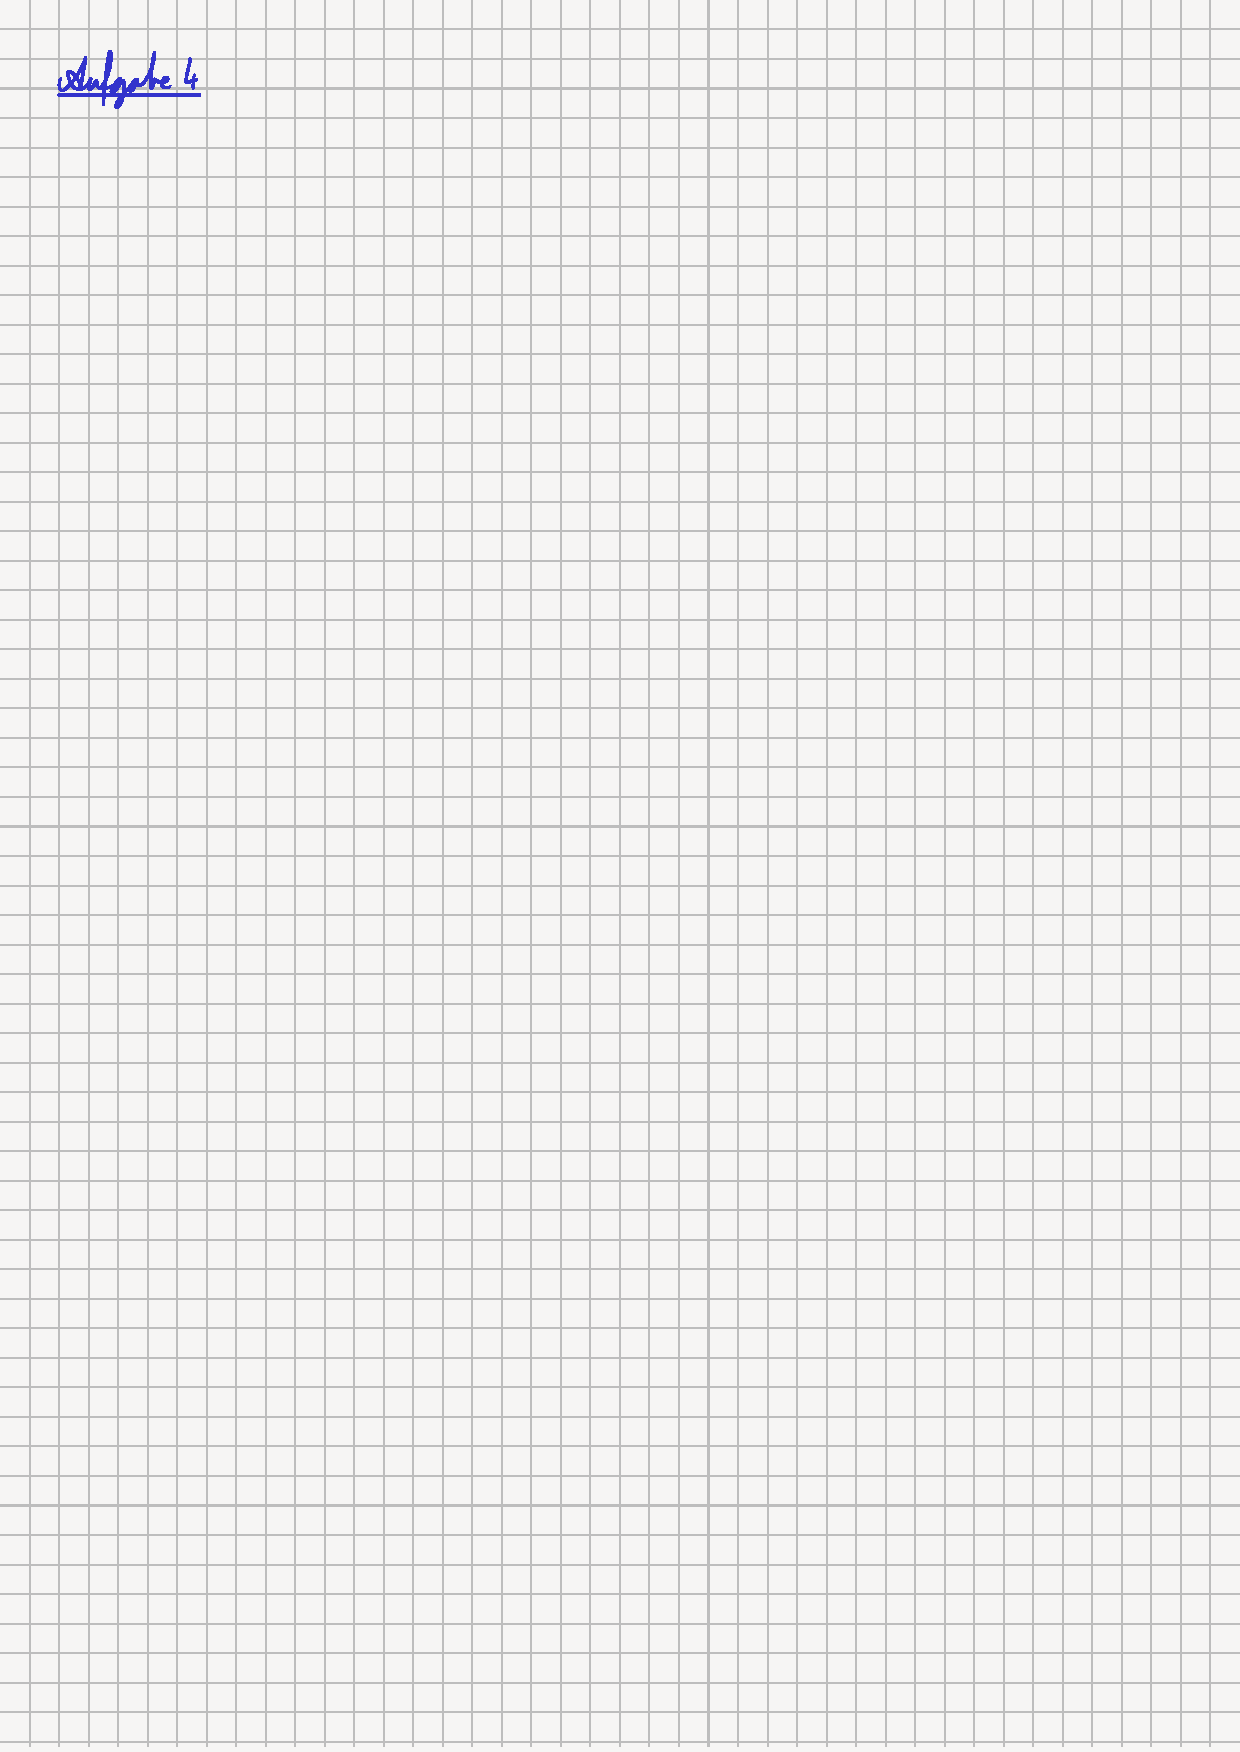
\includepdf[pages=-]{ExampleInput/Aufgabe_4.pdf}




\end{document}
